

\chapter{Examples of utilization}

This section presents some systems that are analyzed and simulated using $SimHPN$.

\section{An assembly line}
\label{s:assembly}

The Petri net system in Fig.~\ref{cas:f-fmsmod} represents an
assembly line with kanban strategy (see~\cite{ZRS-JIM-01}). The
system has two stages that are connected by transition $t_{14}$.
The first stage is composed of three lines (starting from $p_2$,
$p_3$ and $p_4$ respectively) and three machines ($p_{23}$,
$p_{24}$ and $p_{25}$). Places $p_{26}$, $p_{27}$ and $p_{28}$ are
buffers at the end of the lines. The second stage has two lines
that require the same machine/resource $p_{18}$. The number of
kanban cards is given by the marking of places $p_2$, $p_3$ and
$p_4$ for the first stage, and by the marking of $p_{32}$ for the
second stage. The system demand is given by the marking of $p_1$.
We will make use of this net system to illustrate some of the
features of $SimHPN$.

\begin{figure*}[!hbt]
\psfrag{t1}{$t_1$}\psfrag{t2}{$t_2$}\psfrag{t3}{$t_3$}\psfrag{t4}{$t_4$}\psfrag{t5}{$t_5$}\psfrag{t6}{$t_6$}
\psfrag{t7}{$t_7$}\psfrag{t8}{$t_8$}\psfrag{t9}{$t_9$}\psfrag{t10}{$t_{10}$}\psfrag{t11}{$t_{11}$}\psfrag{t12}{$t_{12}$}
\psfrag{t13}{$t_{13}$}\psfrag{t14}{$t_{14}$}\psfrag{t15}{$t_{15}$}\psfrag{t16}{$t_{16}$}\psfrag{t17}{$t_{17}$}\psfrag{t18}{$t_{18}$}
\psfrag{t19}{$t_{19}$}\psfrag{t20}{$t_{20}$}\psfrag{t21}{$t_{21}$}
\psfrag{p1}{$p_1$}\psfrag{p2}{$p_2$}\psfrag{p3}{$p_3$}\psfrag{p4}{$p_4$}\psfrag{p5}{$p_5$}\psfrag{p6}{$p_6$}\psfrag{p7}{$p_7$}
\psfrag{p8}{$p_8$}\psfrag{p9}{$p_9$}\psfrag{p10}{$p_{10}$}\psfrag{p11}{$p_{11}$}\psfrag{p12}{$p_{12}$}\psfrag{p13}{$p_{13}$}\psfrag{p14}{$p_{14}$}
\psfrag{p15}{$p_{15}$}\psfrag{p16}{$p_{16}$}\psfrag{p17}{$p_{17}$}\psfrag{p18}{$p_{18}$}\psfrag{p19}{$p_{19}$}\psfrag{p20}{$p_{20}$}\psfrag{p21}{$p_{21}$}
\psfrag{p22}{$p_{22}$}\psfrag{p23}{$p_{23}$}\psfrag{p24}{$p_{24}$}\psfrag{p25}{$p_{25}$}\psfrag{p26}{$p_{26}$}\psfrag{p27}{$p_{27}$}\psfrag{p28}{$p_{28}$}
\psfrag{p29}{$p_{29}$}\psfrag{p30}{$p_{30}$}\psfrag{p31}{$p_{31}$}\psfrag{p32}{$p_{32}$}
    \centering{
         {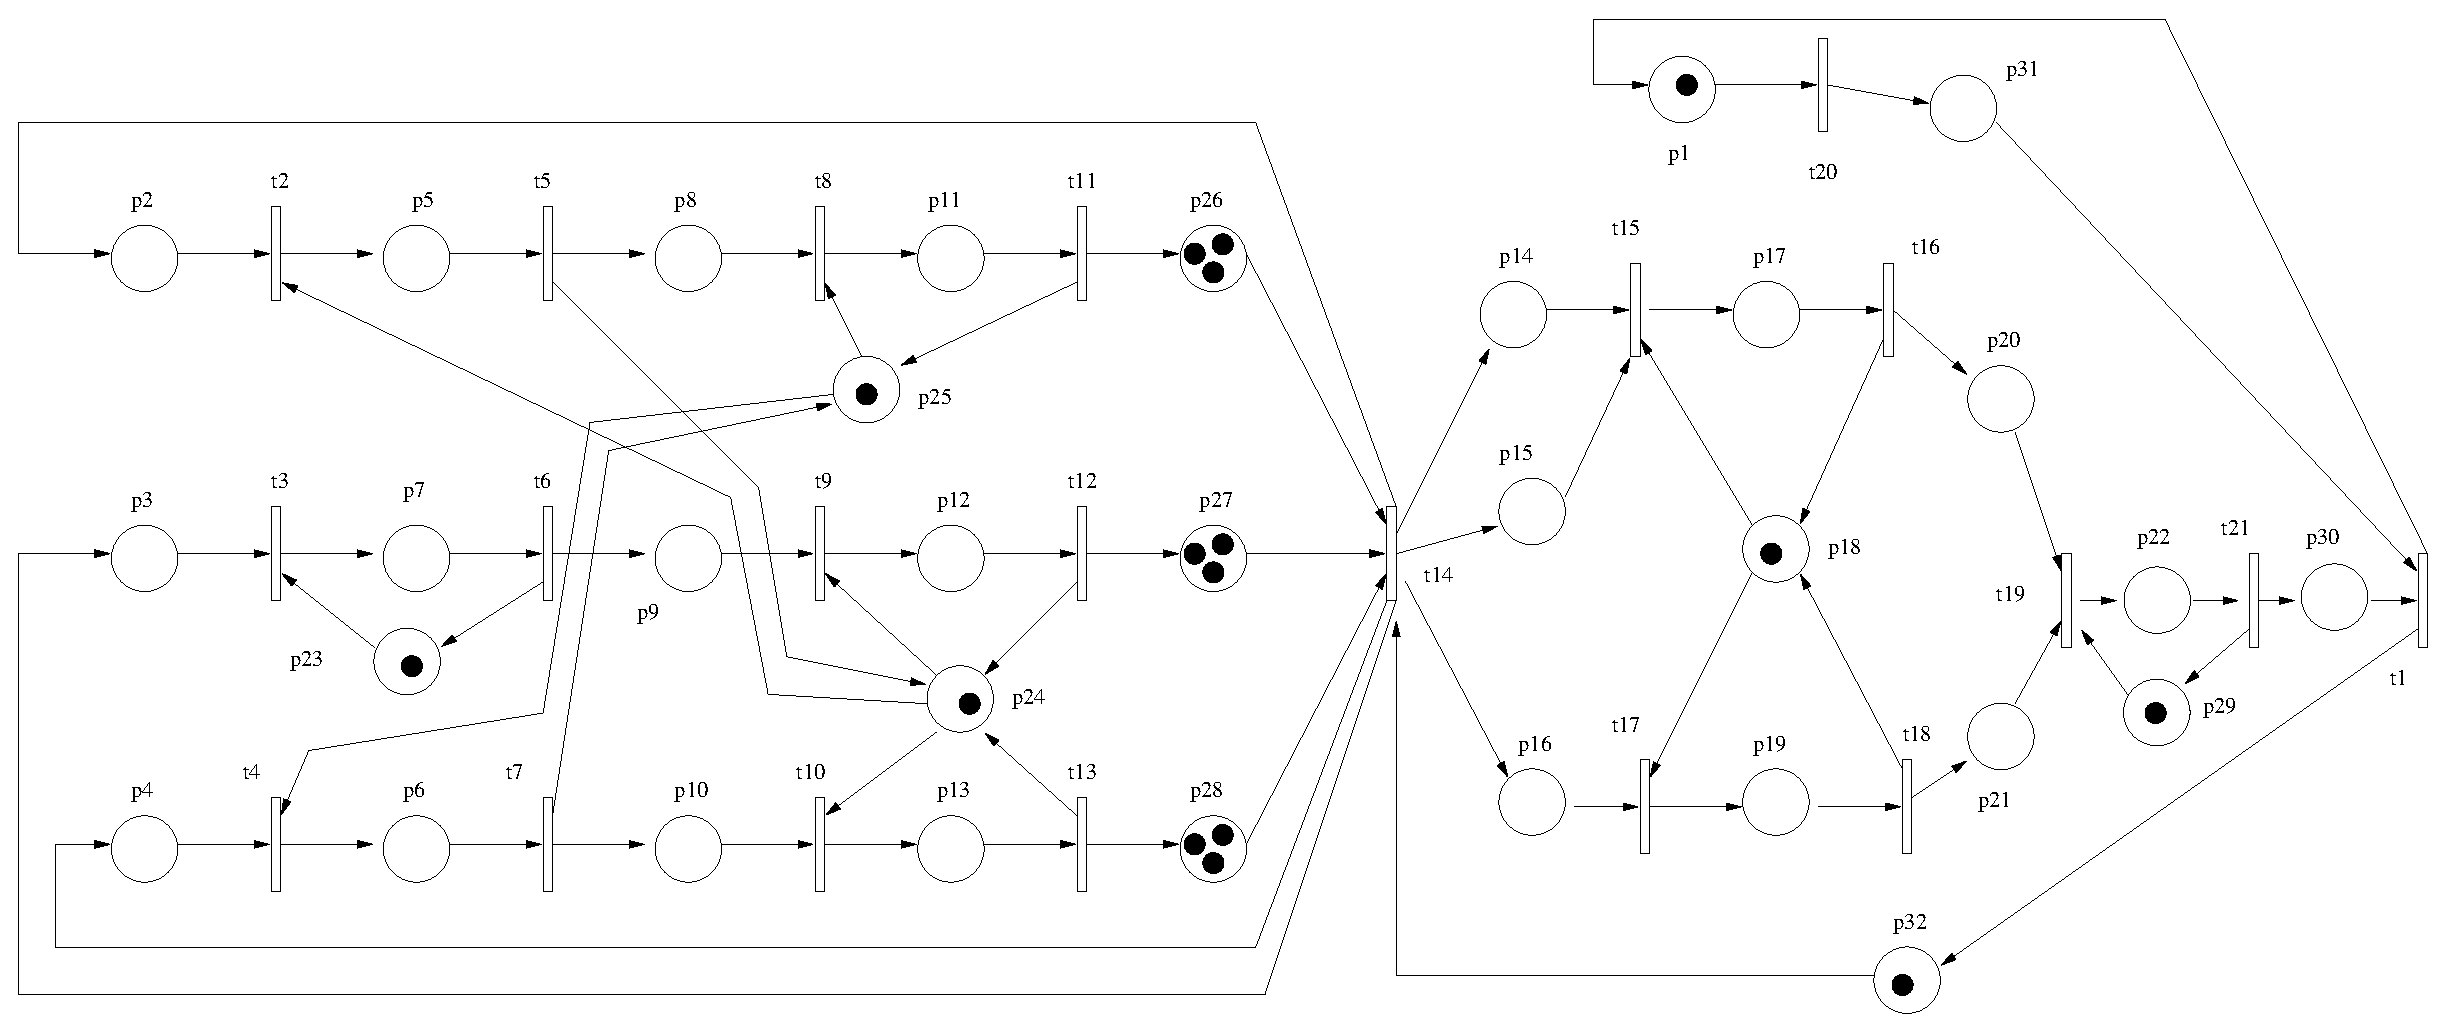
\includegraphics[width=0.95\linewidth] {figs/fmsmodi.eps}}
       }
    \caption[]{An assembly line with kanban strategy.}
   \label{cas:f-fmsmod}
\end{figure*}

Given that all transitions represent actions that can potentially have
high working loads, all transitions are considered continuous.
Moreover, infinite server semantics will be adopted for all of them. Let
the initial marking be $\mo(p_1)=\mo(p_{18})=\mo(p_{23})=\mo(p_{24})=\mo(p_{25})=\mo(p_{29})=\mo(p_{32})=1$,
$\mo(p_{26})=\mo(p_{27})=\mo(p_{28})=3$ and the marking of the
rest of places be equal to zero. Let us assume that the firing rates of the transitions are
$\la(t_2)=\la(t_3)=\la(t_4)=\la(t_8)=\la(t_9)=\la(t_{10})=\la(t_{14})=\la(t_{15})=\la(t_{17})=\la(t_{19})=\la(t_{20})=10$,
$\la(t_1)=\la(t_5)=\la(t_6)=\la(t_7)=\la(t_{11})=\la(t_{12})=\la(t_{13})=\la(t_{16})=\la(t_{18})=\la(t_{21})=1$.

{\bf Computation of minimal P-T \emph{semiflows}:} $SimHPN$ implements
the algorithm proposed in~\cite{BOSilv85} to compute the minimal P-\emph{semiflows} of a Petri net. The same algorithm applied on the transpose of the incidence matrix yields the minimal T-\emph{semiflows} of the net. Notice that P and T-\emph{semiflows}
just depend on the structure of the net and not on the continuous or discrete
nature of the transitions. The result of applying the algorithm on the net
in Fig.~\ref{cas:f-fmsmod} is the set of  $12$ minimal P-semiflows that
cover every place, i.e., it is conservative, and the set that contains the only
minimal T-semiflow  which is a vector of ones, i.e., it is consistent.


{\bf Throughput bounds:}  When all transitions are continuous and work
under infinite server semantics, the following programming problem can be used to compute an upper bound for the throughput, i.e., flow,  of a transition (\cite{ARJuReSi05}):
\begin{equation}
\begin{array}{l}
\max \{ \phi_j \ |\ \b{\mu}^{ss} = \mo + \b{C} \cdot \b{\sigma}, \\
\ \ \ \ \ \ \phi^{ss}_j = \lambda_j \cdot \min \limits_{p_i \in \preset{t_j}} \left\{ \frac{\mu^{ss}_i}{Pre(p_i,t_j)}  \right\}, \forall t_j \in T, \\
\ \ \ \ \ \ \b{C} \cdot \phi^{ss} = \b{0}, \\
\ \ \ \ \ \ \b{\mu}{ss}, \b{\sigma} \geq \b{0} \}.
\end{array}
\end{equation}
This non-linear programming problem is difficult to solve due to the minimum operator. When a transition $t_j$ has a single input place, the equation reduces to \eqref{eqeg}. And when $t_j$ has more than an input place, it can be relaxed (linearized) as \eqref{eqin}.

\begin{equation}
\label{eqeg}
\phi^{ss}_j = \lambda_j \cdot \frac{\mu^{ss}_i}{Pre(p_i,t_j)}, \mbox{if\ } p_i=\preset{t_j}
\end{equation}

\begin{equation}
\label{eqin}
\phi^{ss}_j \leq \lambda_j \cdot \frac{\mu^{ss}_i}{Pre(p_i,t_j)}, \forall p_i \in \preset{t_j}, \mbox{otherwise}
\end{equation}

This way we have a single linear programming problem, that can be solved in polynomial time.
Unfortunately, this LPP provides in general a non-tight bound, i.e., the solution may be non-reachable for any distribution of the tokens verifying the P-\emph{semiflow} load conditions, $\b{y} \cdot \mo$. One way to improve this bound is to force the equality for at least one place per synchronization (a transition with more than one input place). The problem is that there is no way to know in advance which of the input places should restrict the flow. In order to overcome this problem, a branch \& bound algorithm can be used to compute a reachable steady state marking.

$SimHPN$ implements such a branch \& bound algorithm to compute upper throughput
bounds of continuous nets under infinite server semantics. For the system in
Fig.~\ref{cas:f-fmsmod} with the mentioned $\mo$ and $\la$ the obtained
throughput bound for $t_1$ is $0.3030$. Given that the only T-semiflow of the
net is a vector of ones, this value applies as an upper bound for the rest of
transitions of the net.

{\bf Optimal Sensor Placement:}
%Assuming that each place can be measured at a different cost, the optimal sensor placement problem of continuous Petri Nets under infinite server semantics is to decide the set of places to be measured such that the net system is observable at minimum cost. Measuring a place allows the observation of a set of others (''covered'' by that measure) but, the problem is not a simple covering one (\cite{SCP79}). The question is studied at the structural level in (\cite{IPMaReSi05}) and the results obtained are used in the implementation of an algorithm to reduce the computational burden. For this net, measuring all input places in synchronization transitions the net system is observable. This is also the solution of the optimal sensor placement problem for any cost associated to transitions.

Assuming that each place $p$ can be measured at a different cost  $c(p) > 0$  the optimal sensor placement problem of continuous nets under infinite server semantics is to decide the set of places $P_o \subseteq P$ to be measured such that the net system is observable at minimum cost. This problem can be seen as a Set Covering Problem which is NP-hard in the strong sense \cite{SCP79}. For a set of places $P_o$, let $K_{P_o}$ be the set of observable places. It will be said that $P_o$ is covering $K_{P_o}$. The problem is to determine a set $P_{o_i}$ with minimum cost such that the covered elements contain all the places of the net.

Considering that $n$ is the number of places, the brute force approach to solve this problem is to try all subsets of places of size $n$, $n-1$, $\cdots$, $1$.  From those subsets ensuring the observability of the continuous Petri net system, the one with minimum cost is taken. In order to reduce the number of the subsets, some graph-based properties can be used. The idea is to group the set of places in equivalence classes such that only one place per  class can belong to the optimal solution.  These equivalence classes are called \emph{threads} and are the places belonging to the maximally connected subnets finishing in an attribution place (place with more than one input transitions) or in a join (transition with more than one input place). Initially, all places of the net belong only to one thread. The following algorithm can be used to reduce the number of elements from threads.



These reductions preserve the optimality of the solution and the covering problem can be started using the resulted threads. It is necessary to generate all combinations taking at most one place from each thread and then check the observability of the system. If the system is observable, the solution is kept if has a cost lower than the candidate solution. A good choice is starting with the first places of each thread and going backward since the following property is true: if the system is not observable for the current
set of measured places, it is not necessary to advance in the threads because the system will not be observable.

The algorithm is still exponential but the structural properties presented can reduce drastically the number of observability checks. For the continuous nets considered in this section, measuring all input places in join transitions the net system is observable. This is also the solution of the optimal sensor placement problem for any cost associated to transitions.



{\bf Optimal Steady-State:}
The only action that can be performed on a continuous Petri nets is to slow down the flow of its transitions. If a transition can be controlled (its flow reduced or even stopped), we will say that is a \textit{controllable} transition. The forced flow of a controllable transition $t_j$ becomes $f_j - u_j$, where $f_j$ is the flow of the unforced system, i.e. without control, and $u_j$ is the control action $0 \leq u_j \leq f_j$.

In production control is frequent the case that the profit function depends on production (benefits in selling), working process and amortization of investments. Under linear hypothesis for fixed machines, i.e., $\b{\lambda}$ defined, the profit function may have the following form:

\begin{equation}
\mathbf{w}^T \cdot \b{f} - \b{z}^T \cdot \b{m} - \b{q}^T \cdot \mo
\end{equation}

where $\b{f}$ is the throughput vector, $\b{m}$ the average marking, $\b{w}$ a gain vector w.r.t. flows, $\b{z}^T$ is the cost vector due to immobilization to maintain the production flow and $\b{q}^T$ represents depreciations or amortization of the initial investments.

The algorithm used to compute the optimal steady state flow (and marking) is very much alike the one used to compute the performance bounds, with the difference that the linear programming problem that needs to be solved is:

\begin{equation}
\left\{
\begin{array}{l}
\max \{ \b{w}^T \cdot \b{f} - \b{z}^T \cdot \b{\m} - \b{q}^T \cdot \mo \ | \ \b{C} \cdot \b{f} = 0, \\
\ \ \ \ \ \ \ \b{m} = \mo + \b{C} \cdot \b{\sigma}, \\
\ \ \ \ \ \ \ f_j = \lambda_j \cdot \left( \frac{m_i}{Pre(p_i,t_j)} \right) - v(p_i,t_j), \\
\ \ \ \ \ \ \  \ \ \ \ \ \ \ \forall p_i \in \preset{t_j}, v(p_i,t_j) \geq 0 \\
\ \ \ \ \ \ \ \b{f}, \b{m}, \b{\sigma} \geq 0
\end{array}
\right.
\end{equation}

where $v(p_i,t_j)$ are slack variables. These slack variables give the control action for each transition. For more details on this topic, see (\cite{ARMaRaReSi08}).

\section{A traffic system}
\label{s:traffic}

Here, a hybrid PN model, that represents a traffic system consisting
of two (one-way streets) intersections connected by a (one-way
street) link, is introduced and simulated. The proposed example is
shown in fig. \ref{f-traffic} (studied in \cite{IPVaSuBoSi10} for
control purposes). In this, the dynamic of the vehicles is
represented by continuous nodes, while the traffic lights are
modeled as discrete.

Let us firstly explain the model of one intersection. Places
$\{p_1^1,p_2^1\}$ represent the queues of vehicles before crossing
the intersection $1$. Cars arrive through $\{t_1^1,t_3^1\}$, being
transitions of type ic constrained by self-loops $\{p_3^1,p_4^1\}$
that represent the number of servers (street lanes). Vehicles depart
through $t_2^1$ or $t_4^1$ (type \emph{ic}) when the traffic light enabled
them, i.e., when there is a token in $p_5^1$ or $p_7^1$,
respectively. The traffic light for this intersection is represented
by nodes $\{p_5^1,p_6^1,p_7^1,p_8^1,t_5^1,t_6^1,t_7^1,t_8^1\}$,
which describe the sequence of the traffic light stages. In this,
the transitions are of type dd. A token in $p_5^1$ means a green
signal for the queue $p_1^1$, but red for $p_2^1$.

Similarly, a
token in $p_7^1$ represents a green signal for the queue $p_2^1$ but
red for $p_1^1$. Places $p_6^1$ and $p_8^1$ represent intermediate
stages when the traffic light is amber for one queue but red for
the other, so no car can cross the intersection. Similarly, nodes
with the superscript $2$, i.e., $\{p^2_x,t^2_x\}$), represent the
nodes of the second intersection and its traffic light. In this, the
place $p_9^2$ and the transition $t_9^2$ (type \emph{dd}) have been added
in order to simulate the offset, i.e., the relative time between the
cycles of both traffic lights, which is given by the delay of
$t_9^2$. The output flow of intersection $1$ feeds the second one
through a link, which imposes a constant delay (given by the delay
of $t_{11}$). A detailed explanation of the link model can be found
in \cite{IPVaSuBoSi10}. Let us just mention here that, due to the
traffic light, vehicles departing intersection $1$ describe a
bursting signal (like platoons or batches of cars) that arrives to
the second intersection through $t_1^2$.


Let us consider the following delays: for
$\{t_5^1,t_6^1,t_7^1,t_8^1\}$ the delays are $(20,5,20,4)$ seconds
(in the same order). For $\{t_1^1,t_2^1,t_3^1,t_4^1\}$ are
$(1,1/3,1/3,1/5)$ seconds, for $\{t_1^2,t_2^2,t_3^2,t_4^2\}$ are
$(1/3,1/5,1,1/3)$ seconds, and for the link
$\{t_9,t_{10},t_{11},t_{12}\}$ are $(1/10,1/3,30,1/3)$ seconds (the
link delay is $\theta_{11}=30$ seconds). The initial marking is as
described in fig. \ref{f-traffic}.


\begin{figure*}
\centering \subfigure[]{
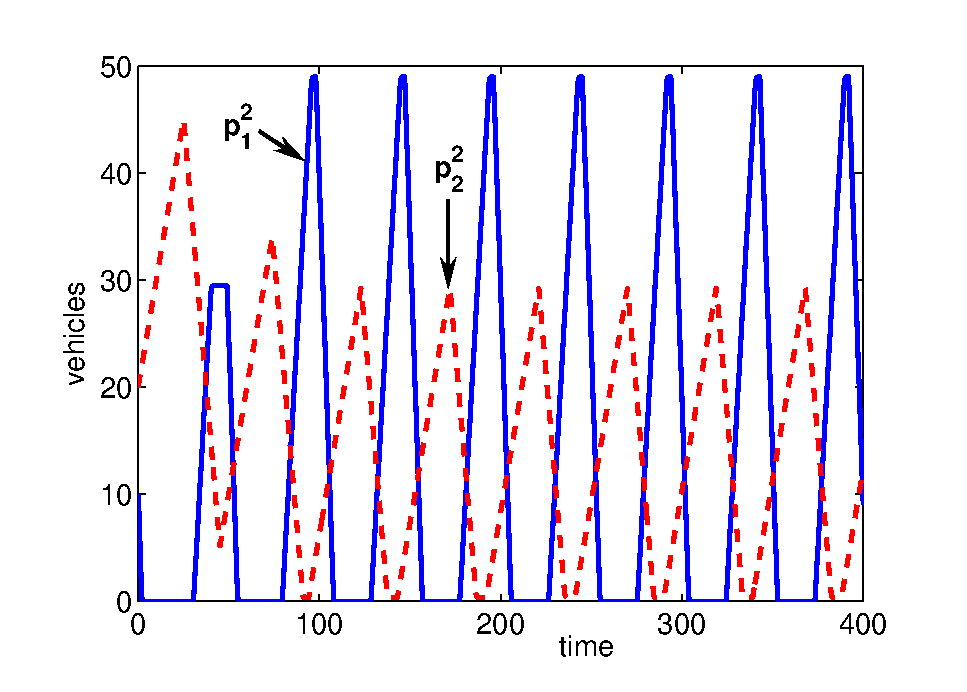
\includegraphics[width=.42\textwidth]{figs/traffic1}}
\hspace{0.5cm} \subfigure[]{
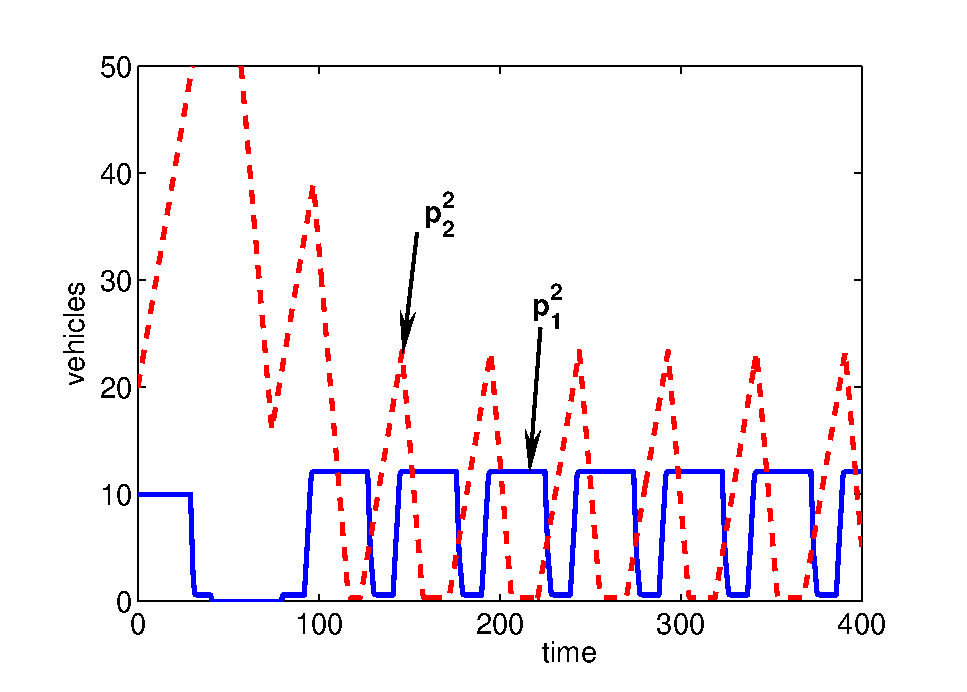
\includegraphics[width=.42\textwidth]{figs/traffic4}}
\caption{Queue lengths at intersection $2$ obtained with delays for
$\{t_5^2,t_7^2,t_9^2\}$ as  a) $\{20,20,0.1\}$ and b)
$\{14,26,29\}$. } \label{ftraficsim}
\end{figure*}

The goal in this example is to obtain, through simulations, suitable
switching delays for the second traffic light, in order to reduce
the queue lengths at intersection $2$. The parameters to optimize
are the green periods (amber periods are fixed and equal to
$\theta_{6}^2=5$ and $\theta_{8}^2=4$), i.e., the delays of $t_5^2$,
$t_7^2$ , and the offset represented by the delay of $t_9^2$. Fig.
\ref{ftraficsim} shows the evolution of the queues for the first 400
seconds, for two cases: a) with green periods $20$ seconds
and no offset, and b) with green periods $14$ for the queue $p_1^2$
and $26$ for the queue $p_2^2$ and with an offset of $29$ seconds.
Note that the second combination of parameters provide shorter
queues. For this, the effect of the offset is very important. This
example shows that simulations based on hybrid PN models can provide
information about the optimal parameters for traffic lights
(duration of stages and offset), in order to improve the performance
in neighboring traffic intersections.


\section{A biochemical system}
\label{s:pathway}

This section presents and simulates a biochemical system modeled by continuous
Petri nets. In most chemical models, the different amounts of chemical substances are expressed
in terms of concentrations rather than as whole numbers of molecules. This implies
that the state of the system is given by a vector of real numbers, where each component
represents the concentration of a compound.
On the other hand, the dynamics
of most reactions is driven by the mass action law, what roughly implies that the
speed of a reaction is proportional to the product of the concentrations of the
reactants. These facts make continuous Petri nets under product semantics an
appealing modeling formalism for biochemical systems.

\begin{figure*}
   \centering{
   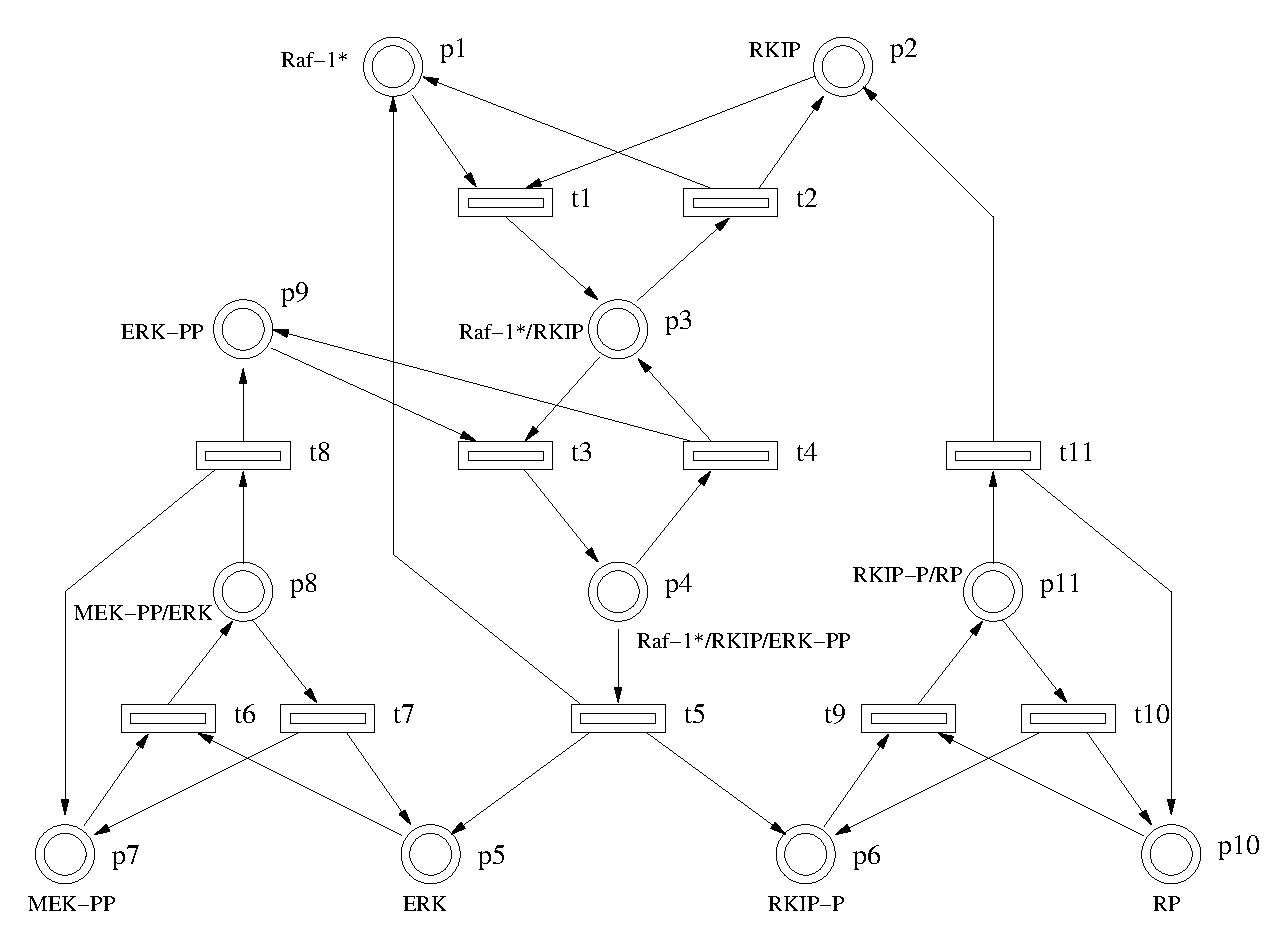
\includegraphics[width=.75\textwidth]{bioches.eps}}
   \caption{Petri net modeling the ERK signaling pathway regulated by RKIP.}
   \label{f:bioches}
\end{figure*}

The net system in Fig.~\ref{f:bioches} models a signaling pathway described and
studied in~\cite{IPChShKi03}. More precisely, the net is a graphical representation
of the Extracellular signal Regulated Kinase (ERK) signaling pathway regulated by
Raf Kinase Inhibitor Protein (RKIP). The marking of each place represents the concentration
of the compound associated to it, and the transitions represent the different
chemical reactions that take place (see~\cite{IPChShKi03} for a more detailed
description of the pathway). Notice that, although the net has conflicts, the assumed 
product semantics fully determines the flows of all continuous transitions,
and therefore it is not necessary to impose a conflict resolution policy.

Since the state of the system is expressed as concentration levels, every transition
is considered continuous and product server semantics is adopted. The parameter
$\b{\lambda}$ estimated in~\cite{IPChShKi03} is
$\b{\lambda}= [0.53,$ $0.0072,$ $0.625,$ $0.00245,$ $0.0315,$ $0.8,$ $0.0075,$ $0.071,$ $0.92,$ $0.00122,$ $0.87]$.
As initial concentrations of the compounds we take the following values:
$\mo=[2,\ 2.5,\ 0,\ 0,\ 0,\ 0,\ 2.5,\ 0,\ 2.5,\ 3,\ 0]$.

\begin{figure}
   \centering{
   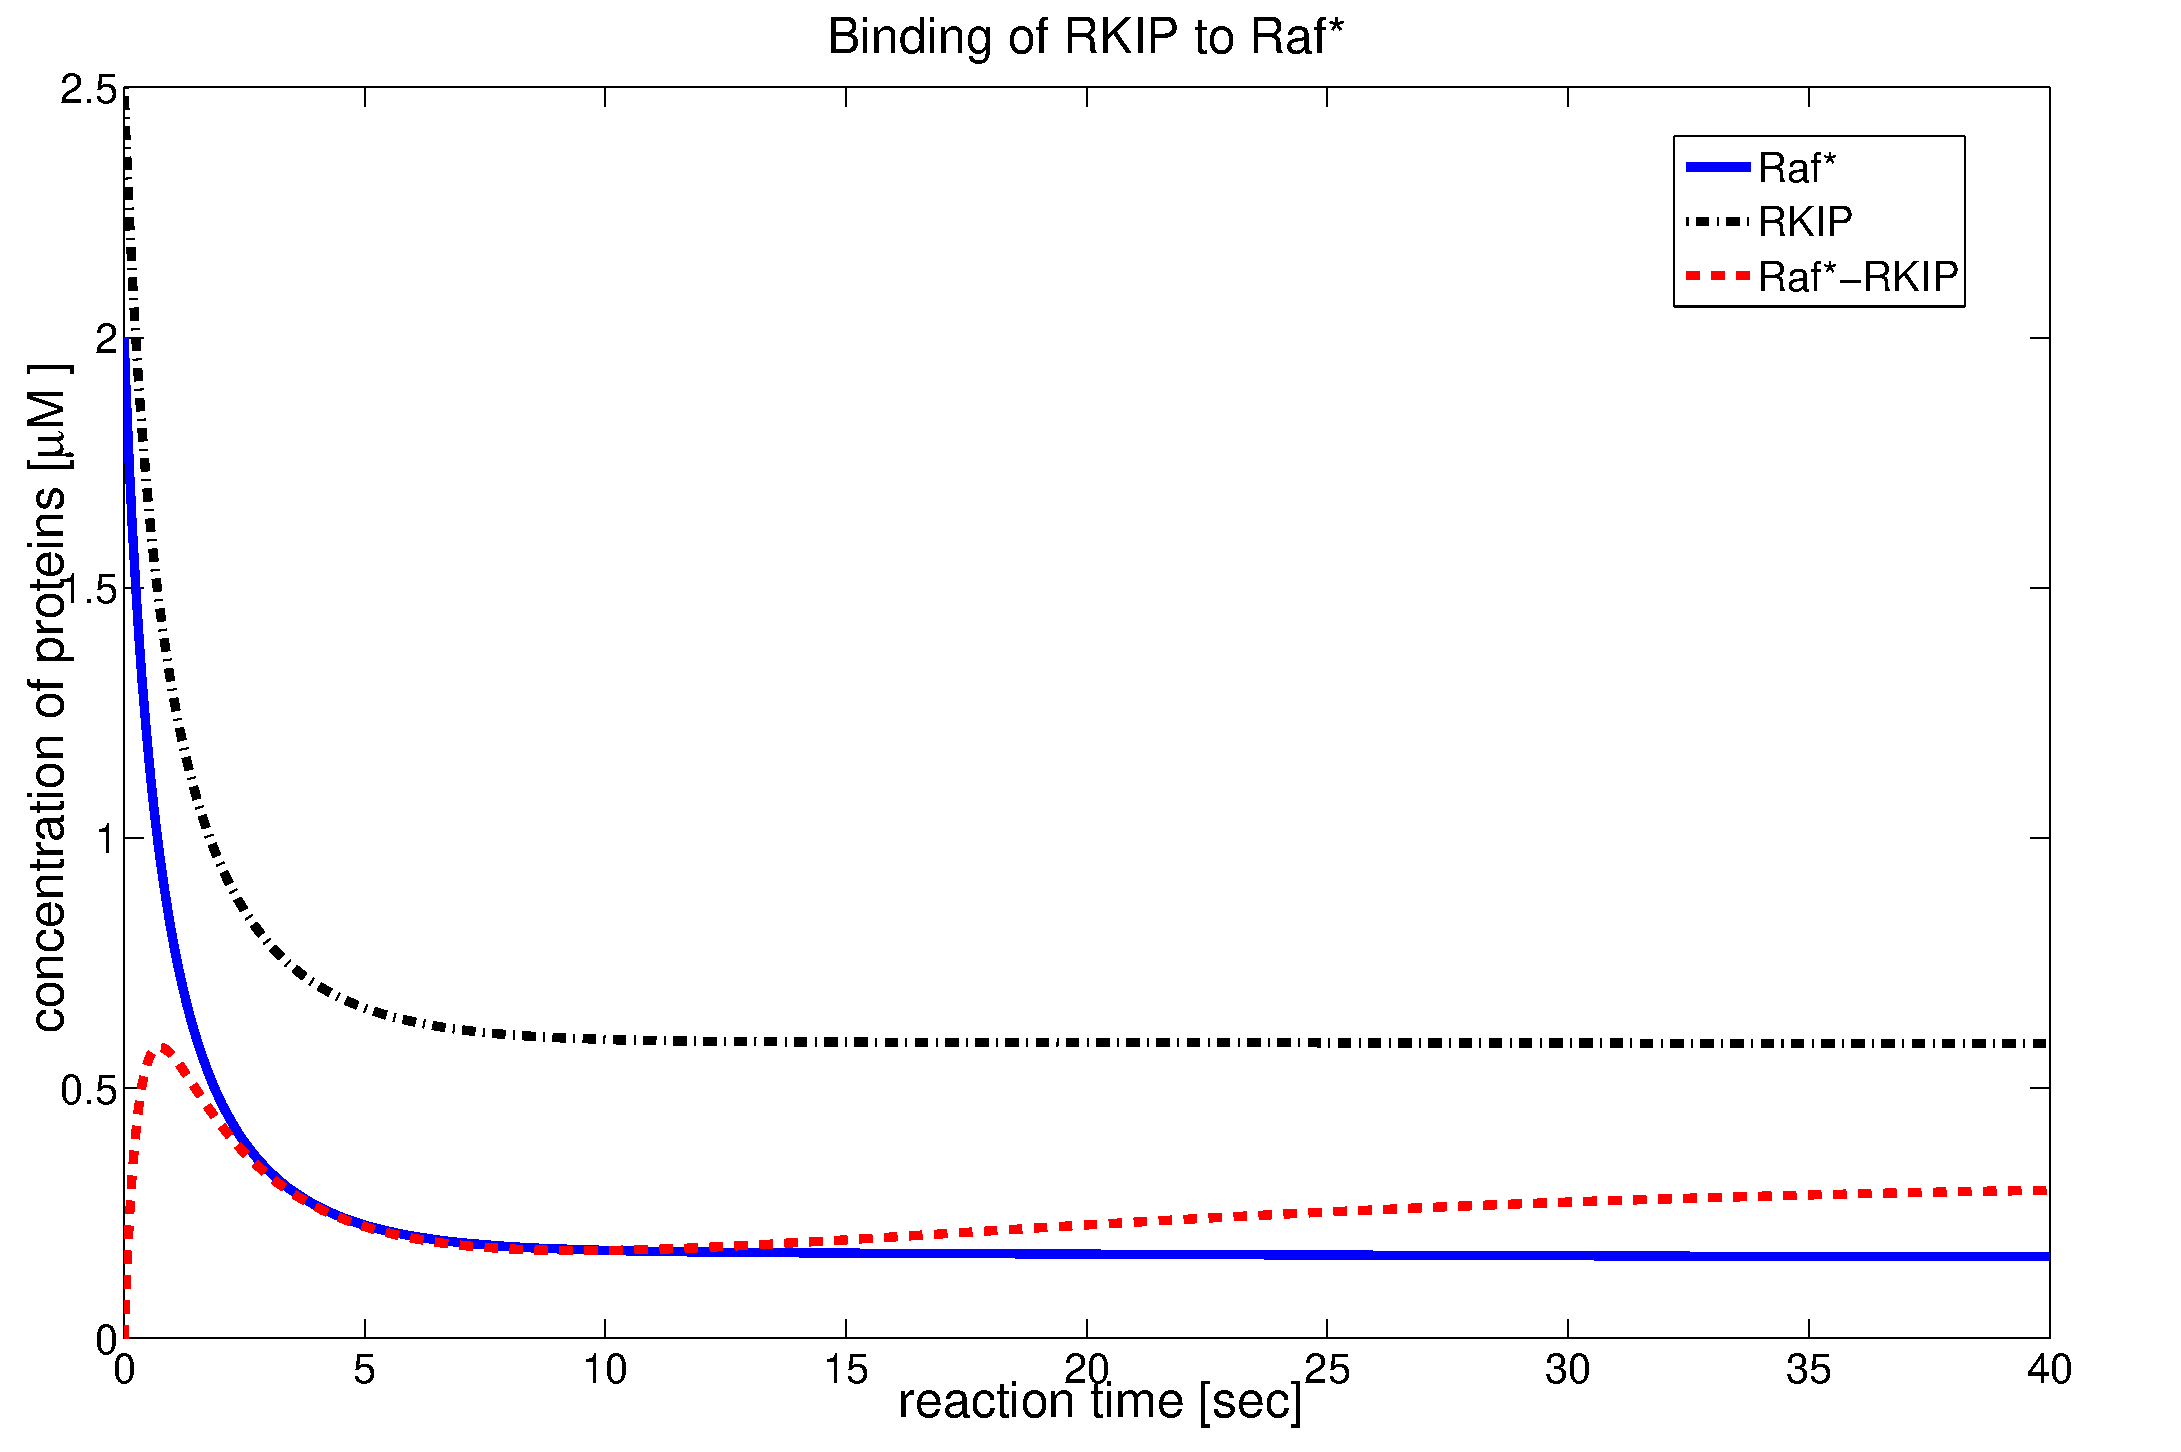
\includegraphics[width=.7\columnwidth]{mf1c1.eps}}
   \caption{Time evolution of Raf-1*, RKIP and their complex Raf-1*/RKIP.}
   \label{f-mf1c1}
\end{figure}

\begin{figure}
   \centering{
   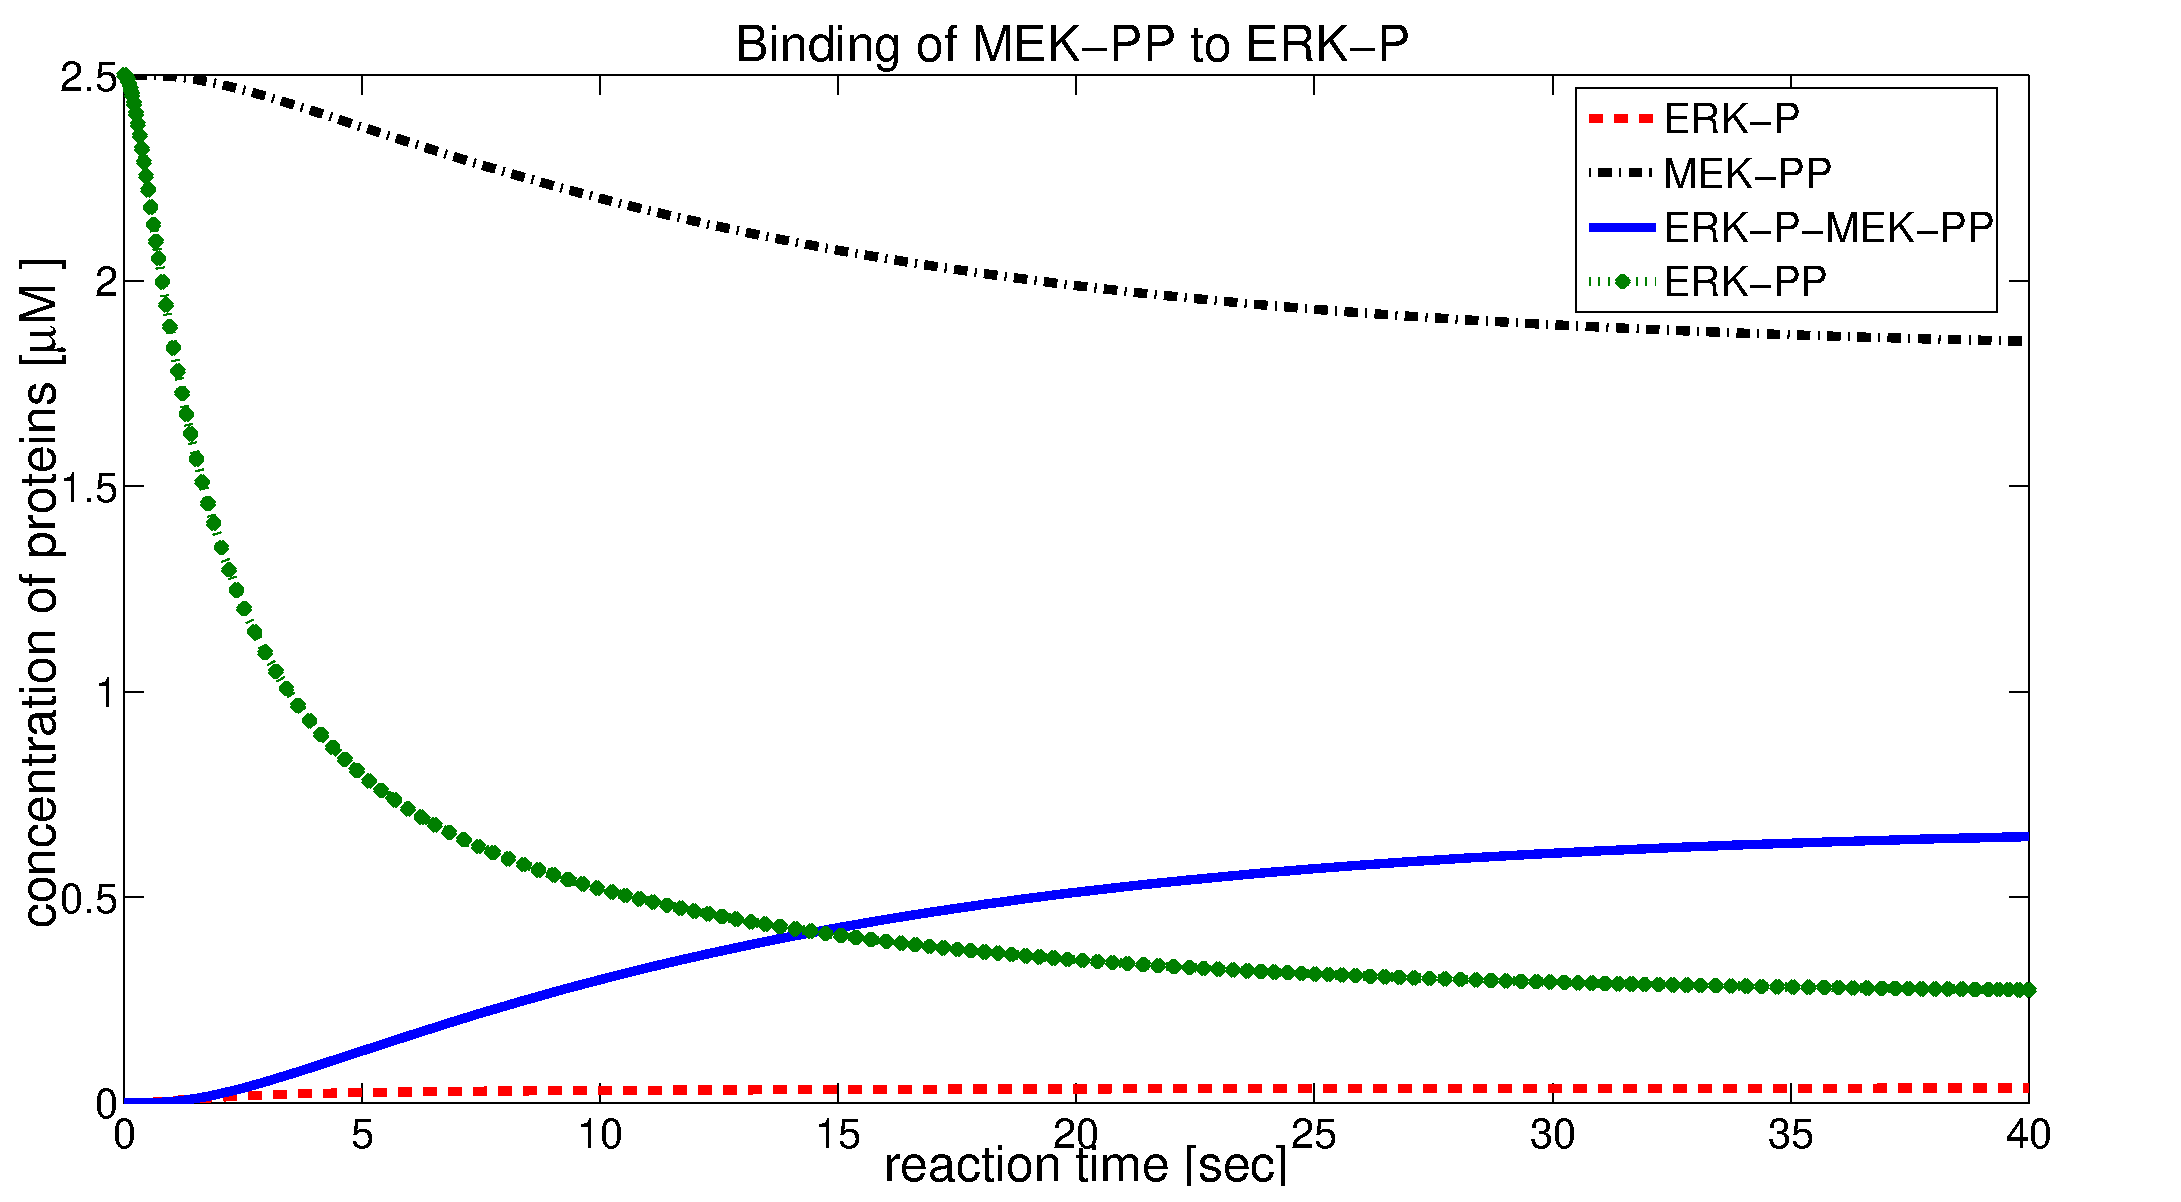
\includegraphics[width=.7\columnwidth, height=6cm]{mf1c2.eps}}
   \caption{Activity of MEK-PP which phosphorylates and activates ERK.}
   \label{f-mf1c2}
\end{figure}

Figures~\ref{f-mf1c1} and ~\ref{f-mf1c2} show the time evolution of some
of the compounds in the system along $40$ time units. In particular, Fig.~\ref{f-mf1c1}
shows the dynamics of Raf-1*, RKIP and their complex Raf-1*/RKIP, and
Fig.~\ref{f-mf1c2} shows the activity of MEK-PP which phosphorylates and activates ERK.
As discussed in~\cite{IPChShKi03}, intensive simulations can be used to
perform sensitivity analysis with respect to the variation of initial conditions.




%%%%%%%%%%%%%%%%%%%%%%%%%%%%%

\section{A Kanban-like flexible manufacturing system}


Here, we consider the Kanban-like flexible manufacturing system (FMS) consisting of two workflows that are attended by a pool of three machines (see Fig. \ref{fig:layoutFINAL}), to perform a structural controllability analysis. A TCPN that models the system is presented in Fig. \ref{fig:FMSPN} (this model is available in the models folder as Model\_FMS\_3.mat). It has 216 configurations and 11 transitions, each one representing one of the following events:
\begin{itemize}
    \item Loading of material to the machines ($t_1,t_3,t_5,t_7,t_9$).
    \item Unloading of the processed material to be stored in a buffer ($t_2,t_4,t_6,t_8,t_{10}$).
    \item Removing parts from the system output ($t_{11}$).
\end{itemize}
The timing of the net is given by $\lambda = \left [1 \ \frac{1}{3} \ 1 \ \frac{1}{4} \ 1 \ \frac{1}{3} \ 1 \ \frac{1}{5} \ 1 \ \frac{1}{5} \ 1 \right ]^T$. 
We work based on the assumption that machines are consistently working at their nominal speed and are freed up as soon as the material is processed. As a result, we have identified $T_{nc}=\{t_2,t_4,t_6,t_8,t_{10}\}$. The remaining events are controllable because it is possible to decide when to use a specific machine to process a particular piece, and we can always empty the output buffer. This leads to $T_c$ being $T_{c}=\{t_1,t_3,t_5,t_7,t_{9},t_{11}\}$.

\begin{figure}[htbp]
    \centering
    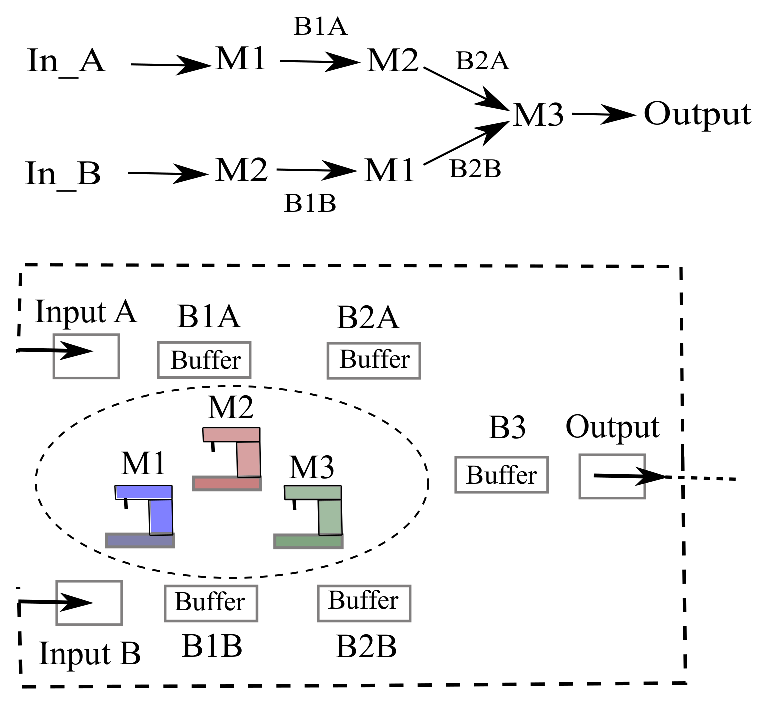
\includegraphics[scale=.6]{figs/FinalExampleLayout2.eps}
    \caption{A Kanban-like flexible manufacturing system. and its production process.}
    \label{fig:layoutFINAL}
\end{figure}

\begin{figure}[htbp]
    \centering
    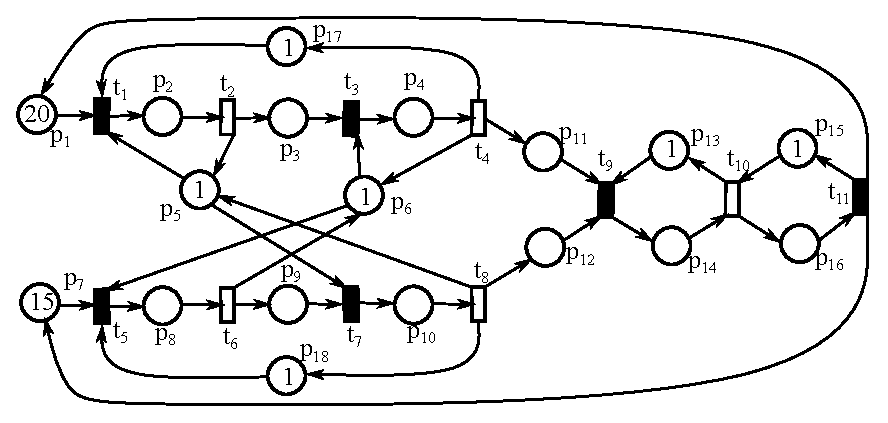
\includegraphics[scale=.75]{figs/FMS.eps}
    \caption{A TCPN system that models the FMS of Fig \ref{fig:layoutFINAL}. The controllable transitions are depicted as black transitions.}
    \label{fig:FMSPN}
\end{figure}

\textbf{Net rank-controllability analysis:} Once the model has been loaded, the test can be carried out by selecting \textit{Continuous} $\rightarrow$ \textit{Structural controllability analysis} $\rightarrow$ \textit{Net rank-controllability test}. We present 3 cases:\\
${\bullet}$ $T_c = \{t_1,t_5\}$: We enter this set of controllable transitions on the pop-up windows as $[1 \ 5]$ and we obtain the message \\``\textit{Influence is not total! Therefore, the set of controllable transitions does not guarantee net rank-controllability. The only influenced nodes are:}
\textit{Places = [1 2 3 4 5 6 7 8 9 10 11 12 17 18]}
\textit{Transitions = [1 2 3 4 5 6 7 8]}'' \\This means that, since the property of influence does not hold, then there are configurations in which the net is not rank-controllable.\\
${\bullet}$ $T_c = \{t_1,t_5,t_9,t_{11}\}$ By entering this set of controllable transitions as $[1 \ 5 \ 9 \ 11]$ we obtain the message \\``\textit{It is not possible to decide if the timed net is net rank-controllable. The condition related to the choice places is not fulfilled.}''. \\In this case the test cannot conclude if the system is NRC, since one of the sufficient conditions does not hold. In particular, the one related to the choice places. This serves to give indications to the operator/researcher about where the problem may be in order to guarantee controllability.\\
${\bullet}$ $T_c = \{t_1,t_3,t_5,t_7,t_9,t_{11}\}$: Here we choose the set that we will consider in our case study, which is such that it satisfies all the structural conditions for controllability and is indicated by the message:
``\textit{The timed net is net rank-controllable.}''.

From the previous analysis, we conclude that the system is NRC. Moreover, this system is a live and bounded TCPN. Therefore, $T_c$ also guarantees that the system will be controllable over its connected sets of equilibrium markings.\\ % For instance, in [14], we have shown how to apply control laws designed for a TCPN into the corresponding Markovian Petri net system.  Once a control law has been designed for a T CP N system, it can be used for controlling the marking of the original discrete net [4


\textbf{Equilibrium connectivity graph: } This routine can be used to calculate the equilibrium connectivity graph of a system by selecting the menu \textit{Continuous} $\rightarrow$ \textit{Structural controllability analysis} $\rightarrow$ \textit{Equilibrium connectivity graph} and entering the set of controllable transitions as the input. Each node of the resulting graph represents a configuration of the system whose region contains equilibrium markings, and the edges indicate the connection between the equilibrium markings of the different regions. This provides insights into the controllability of the system, showing the sets of equilibrium points where the controllability property holds. 


Using this routine and selecting the set of controllable transitions $[1 \ 3 \ 5 \ 7 \ 9 \ 11]$, a matrix E\_conf is obtained. Each row of this matrix represents a configuration of the system in which equilibrium markings are present in the corresponding regions. For this particular case, the results are the following:


E\_conf =\\
     1     2     3     4     7     8     9    10    13    14    16   (node 1) \qquad
     1     2     3     4     7     8     9    10    13    15    16   (node 2)\\
     1     2     3     4    18     8     9    10    12    14    16 (node 3) \qquad
     1     2     3     4    18     8     9    10    12    15    16 (node 4)\\
     1     2     3     4    18     8     9    10    13    14    16 (node 5)\qquad
     1     2     3     4    18     8     9    10    13    15    16 (node 6)\\
    17     2     3     4     7     8     9    10    11    14    16 (node 7)\qquad
    17     2     3     4     7     8     9    10    11    15    16 (node 8)\\
    17     2     3     4     7     8     9    10    13    14    16 (node 9)\qquad
    17     2     3     4     7     8     9    10    13    15    16 (node 10)\\
    17     2     3     4    18     8     9    10    11    14    16 (node 11)\qquad
    17     2     3     4    18     8     9    10    11    15    16 (node 12)\\
    17     2     3     4    18     8     9    10    12    14    16 (node 13)\qquad
    17     2     3     4    18     8     9    10    12    15    16 (node 14)\\
    17     2     3     4    18     8     9    10    13    14    16 (node 15)\qquad
    17     2     3     4    18     8     9    10    13    15    16 (node 16)\\

For instance, the region corresponding to the configuration $\mathcal{C}_1 = \{(p_1,t_1),(p_2,t_2),(p_3,t_3),(p_4,t_4),(p_7,t_5),(p_8,t_6),(p_9,t_7),(p_{10},t_8),(p_{13},t_9)$, $(p_{14},t_{10}),(p_{16},t_{11})\}$ (node 1) contains equilibria. Furthermore, the routine generates a variable-type graph called E\_graph, which has 16 nodes and 76 edges, representing the connectivity of the equilibrium sets. This graph can be plotted (as in Fig. \ref{fig:my_label}), providing a visual representation of the equilibrium connectivity of the system. For this particular case, the equilibrium sets in all the regions are connected, meaning that the system exhibits the controllability property over all of its equilibrium markings. 


\begin{figure}
    \centering
    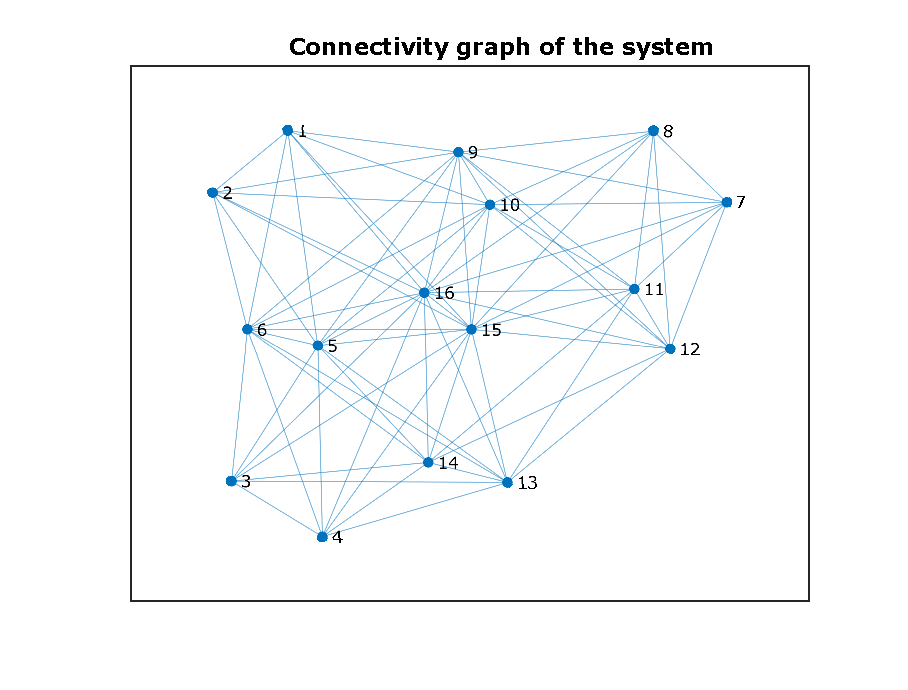
\includegraphics{figs/E_graph.eps}
    \caption{Equilibrium connectivity graph of the FMS system. Each node corresponds to a single region of the TCPN system in which it contains equilibrium markings.}
    \label{fig:my_label}
\end{figure}

%%%%%%%%%%%%%%%%%%%%%%%%%%%%%
\section{Fault Diagnosis with continuous Petri nets}
\label{sec:fdsexamps}

The following examples illustrating the fault diagnosis procedure using untimed continuous Petri nets have been considered in \cite{ARMASECASI12}. 

\subsection{Example 1}
Let us consider the Petri net in Figure~\ref{f-es1} with:
$$T_o=\{t_1, t_2, t_3 \}, \quad T_u=\{ \varepsilon_4, \varepsilon_5, \varepsilon_6, \varepsilon_7,
\varepsilon_8 \} \quad {\text and} \quad T_f^1=\{ \varepsilon_5\}.$$

\begin{figure}[]
\begin{center}
\includegraphics*[scale=.5]{fig1.eps}
\caption[]{The Petri net system considered in Examples~5, 8, 10 and
12 of \cite{ARMASECASI12}.}
   \label{f-es1}
\end{center}
\end{figure}

The matrices $Pre$, $Post$ and $m_0$ can be imported in $SimHPN$ toolbox using
$diagnosis1.mat$ file from the $Models$ folder. Places and transitions follow the
numeration in Figure~\ref{f-es1}. The following input parameters should be used:

\begin{itemize}
\item Number of observable transitions: $3$
\item Sequence of observed transitions: $[ 1 \ 2 \ 3 ]$
\item Sequence of observed firing quantity of transitions: $[0.7 \ 0.5 \ 0.5]$
\item Number of fault classes: $1$
\item Transitions in fault class $1$: $5$
\end{itemize}

In such a case we have only one fault class containing transition
$\varepsilon_5$. Note that, in the matrices $Pre$ and $Post$ the observable transitions have to
occupy the first columns. We are considering the following
observation: $t_1(0.7) t_2(0.5) t_3(0.5)$. The following results are shown at the MATLAB command prompt:

\begin{verbatim}
Number of observable transitions: 3 
First 3 transitions are observable and the rest not
Fault class Tf^{1}={\epsilon_5}

Observed sequence: t1(0.7)t2(0.5)t3(0.5) 
=========================================
==========press a key to continue========
=========================================

Enabling bound of t4 is 2
Enabling bound of t5 is 2
Enabling bound of t6 is 2
Enabling bound of t7 is 2
Enabling bound of t8 is 2

***********************************************************
For empty word:
***********************************************************

Vertices of the set of consistent markings (vertices of \bar Y(m_0,w))
e_1 = [0 1 0 0 0 0 1 0 0 0 0 0]'
e_2 = [0 0 1 0 1 0 1 0 0 1 0 0]'

Computing the diagnosis states
Diagnosis state for Tf^{1}: N

***********************************************************
Observed sequence:  t1(0.70)
***********************************************************

Vertices of the set of consistent markings after cutting
e_1 = [0 0.3 0.7 0 0.7 0 1 0 0 0.7 0 0]'
e_2 = [0 0 1 0 1 0 1 0 0 1 0 0]'
***********************************************************
Vertices of the set of consistent markings (vertices of \bar Y(m_0,w))
e_1 = [0 0 0.3 0 0.3 0 1.7 0 0 1 0 0.7]'
e_2 = [0 0.3 0 0 0 0 1.7 0 0 0.7 0 0.7]'
e_3 = [0 0.3 0 0 0 0.7 1 0 0 0.7 0 0]'
e_4 = [0 0 0.3 0 0.3 0.7 1 0 0 1 0 0]'
Computation time:                 0.01 seconds
Computing the diagnosis states
Diagnosis state for Tf^{1}: N

***********************************************************
Observed sequence:  t1(0.70) t2(0.50)
***********************************************************

Vertices of the set of consistent markings after cutting
e_1 = [0 0.3 0 0 0 0 1.7 0 0 0.7 0 0.7]'
e_2 = [0 0 0.3 0 0.3 0 1.7 0 0 1 0 0.7]'
e_3 = [0 0 0.3 0 0.3 0.7 1 0 0 1 0 0]'
e_4 = [0 0.3 0 0 0 0.7 1 0 0 0.7 0 0]'
***********************************************************
Vertices of the set of consistent markings (vertices of \bar Y(m_0,w))
e_1 = [0 0.3 0.5 0 0.5 0 1.2 0 0.5 0.7 0.5 0.7]'
e_2 = [0.5 0.3 0 0 0 0 1.2 0 0 0.7 0 0.7]'
e_3 = [0 0.3 0.5 0.5 0 0 1.2 0 0.5 0.7 0 0.7]'
e_4 = [0 0.8 0 0 0 0 1.2 0.5 0 0.7 0 0.7]'
e_5 = [0 0 0.8 0 0.8 0 1.2 0.5 0 1.5 0 0.7]'
e_6 = [0 0 0.8 0.5 0.3 0 1.2 0 0.5 1 0 0.7]'
e_7 = [0.5 0 0.3 0 0.3 0 1.2 0 0 1 0 0.7]'
e_8 = [0 0 0.8 0 0.8 0 1.2 0 0.5 1 0.5 0.7]'
e_9 = [0 0 0.8 0 0.8 0.7 0.5 0.5 0 1.5 0 0]'
e_10 = [0 0 0.8 0.5 0.3 0.7 0.5 0 0.5 1 0 0]'
e_11 = [0.5 0 0.3 0 0.3 0.7 0.5 0 0 1 0 0]'
e_12 = [0 0 0.8 0 0.8 0.7 0.5 0 0.5 1 0.5 0]'
e_13 = [0 0.8 0 0 0 0.7 0.5 0.5 0 0.7 0 0]'
e_14 = [0 0.3 0.5 0.5 0 0.7 0.5 0 0.5 0.7 0 0]'
e_15 = [0.5 0.3 0 0 0 0.7 0.5 0 0 0.7 0 0]'
e_16 = [0 0.3 0.5 0 0.5 0.7 0.5 0 0.5 0.7 0.5 0]'
Computation time:                 0.01 seconds
Computing the diagnosis states
Diagnosis state for Tf^{1}: U

***********************************************************
Observed sequence:  t1(0.70) t2(0.50) t3(0.50)
***********************************************************

Vertices of the set of consistent markings after cutting
e_1 = [0 0.3 0.5 0.5 0 0 1.2 0 0.5 0.7 0 0.7]'
e_2 = [0 0 0.8 0.5 0.3 0 1.2 0 0.5 1 0 0.7]'
e_3 = [0 0 0.8 0.5 0.3 0.7 0.5 0 0.5 1 0 0]'
e_4 = [0 0.3 0.5 0.5 0 0.7 0.5 0 0.5 0.7 0 0]'
***********************************************************
Vertices of the set of consistent markings (vertices of \bar Y(m_0,w))
e_1 = [0 0 0.8 0 0.3 0 1.2 0 0.5 1 0 0.7]'
e_2 = [0 0.3 0.5 0 0 0 1.2 0 0.5 0.7 0 0.7]'
e_3 = [0 0.3 0.5 0 0 0.7 0.5 0 0.5 0.7 0 0]'
e_4 = [0 0 0.8 0 0.3 0.7 0.5 0 0.5 1 0 0]'
Computation time:                 0.00 seconds
Computing the diagnosis states
Diagnosis state for Tf^{1}: F
\end{verbatim}

\subsection{Example 2: (a manufacturing system)}

Let us consider the Petri net in Fig.~\ref{model2} where transitions
$t_1$ to $t_{12}$ correspond to observable events, transitions
$\varepsilon_{13}$ to $\varepsilon_{24}$ correspond to unobservable
but regular events while $\varepsilon_{25}$ and $\varepsilon_{26}$
are unobservable and faulty transitions. In particular we assume
$T_f^1=\{\varepsilon_{25}\}$ and $T_f^2=\{\varepsilon_{26}\}$.

\begin{figure*}
\begin{center}
\includegraphics*[scale=0.7]{manufacturing.eps}
\end{center}
\caption{Petri net model of the manufacturing system considered in
Subsection~VII.A.} \label{model2}
\end{figure*}

The matrices $Pre$, $Post$ and $m_0$ are defined in the MATLAB file
$Diagnosis\_2.mat$ and can be imported in $SimHPN$ toolbox using the menu $File\ \rightarrow \ Import\ from\ .mat\ file$. Places and transitions follow the numeration in Fig.~\ref{model2}. The following parameters will be considered:

\begin{itemize}
\item Number of observable transitions: $12$
\item Sequence of observed transitions: $[1  \   1  \   2  \  12 \    3 \    12 \    3  \   6 \    7 \    8  \   4   \  5 \    9\    10  \  11 ]$
\item Sequence of observed firing quantity of transitions: $[1  \   1 \    1 \    1   \  1    \ 1  \   1 \    1  \   1  \   1   \  1  \   1  \   1  \   1 \    1]$
\item Number of fault classes: $1$
\item Transitions in fault class $1$: $[25\ 26]$
\end{itemize}

This net system has two fault classes. The first one contains transition
$\varepsilon_{25}$ and the second one contains transition
$\varepsilon_{26}$. The cardinality of the set of observable
transitions is $12$ and the considered observation is $w= t_1(1)
t_1(1) t_2(1) t_{12}(1) t_3(1) t_{12}(1) t_3(1) t_6(1) t_7(1)t_8(1)
t_4(1) t_5(1) t_9(1) t_{10}(1) t_{11}(1)$. The fault state after each observation is shown at the MATLAB command prompt.

\subsection{Example 3: (unobservable acyclic subnet)}

Let us consider the Petri net in Figure~\ref{fig_new_example2} where
transitions $t_1$ to $t_{6}$ correspond to observable events,
transitions $\varepsilon_{7}$ and $\varepsilon_{8}$ correspond to
unobservable but regular events while $\varepsilon_{9}$ and
$\varepsilon_{10}$ are unobservable and faulty transitions. In
particular we assume $T_f^1=\{\varepsilon_{9}\}$ and
$T_f^2=\{\varepsilon_{10}\}$.

\begin{figure}
\begin{center}
\includegraphics*[scale=0.6]{example2.eps}
\end{center}
\caption{The Petri net considered in Subsection~VII.B.}
\label{fig_new_example2}
\end{figure}

The matrices $Pre$, $Post$ and $m_0$ can be imported from
$Diagnosis\_3.mat$ file. Places and transitions follow the
numeration in Fig.~\ref{model2} and the following parameters are used:

\begin{itemize}
\item Number of observable transitions: $6$
\item Sequence of observed transitions: $[1  \   2  \   5  \  4 \    1 \    3 ]$
\item Sequence of observed firing quantity of transitions: $[0.1   \ 0.1  \  0.3  \  0.1  \ 0.1  \  0.1]$
\item Number of fault classes: $2$
\item Transitions in fault class $1$: $[9]$
\item Transitions in fault class $2$: $[10]$
\end{itemize}


Such net has two fault classes. The first one contains transition
$\varepsilon_{9}$ and the second one contains transition
$\varepsilon_{10}$. The cardinality of the set of observable
transitions is $6$ and the considered observation is $w= t_1(0.1)
t_2(0.1) t_5(0.3) t_{4}(0.1) t_1(0.1) t_{3}(0.1)$. The following
results are obtained at the MATLAB prompt:



\begin{verbatim}
Number of observable transitions: 6 
First 6 transitions are observable and the rest not
Fault class Tf^{1}={\epsilon_9}
Fault class Tf^{2}={\epsilon_10}

Observed sequence: t1(0.1)t2(0.1)t5(0.3)t4(0.1)t1(0.1)t3(0.1) 
=========================================
==========press a key to continue========
=========================================

Enabling bound of t7 is 2.000000e+00
Enabling bound of t8 is 2.000000e+00
Enabling bound of t9 is 2
Enabling bound of t10 is 2.000000e+00

***********************************************************
For empty word:
***********************************************************

Vertices of the set of consistent markings (vertices of \bar Y(m_0,w))
e_1 = [2 2 0 0 0 0 0 0 0 0 0 0]'

Computing the diagnosis states
Diagnosis state for Tf^{1}: N
Diagnosis state for Tf^{2}: N

***********************************************************
Observed sequence:  t1(0.10)
***********************************************************

Vertices of the set of consistent markings after cutting
e_1 = [2 2 0 0 0 0 0 0 0 0 0 0]'
***********************************************************
Vertices of the set of consistent markings (vertices of \bar Y(m_0,w))
e_1 = [1.6 2 0 0 0 0 0.2 0 0.1 0 0.1 0]'
e_2 = [1.6 2 0.1 0 0 0 0.1 0 0.1 0 0 0]'
e_3 = [1.6 2 0.1 0.1 0 0 0 0 0 0 0 0]'
e_4 = [1.6 2 0 0.1 0 0 0.1 0 0 0 0.1 0]'
Computation time:                 0.01 seconds
Computing the diagnosis states
Diagnosis state for Tf^{1}: U
Diagnosis state for Tf^{2}: N

***********************************************************
Observed sequence:  t1(0.10) t2(0.10)
***********************************************************

Vertices of the set of consistent markings after cutting
e_1 = [1.6 2 0.1 0 0 0 0.1 0 0.1 0 0 0]'
e_2 = [1.6 2 0 0 0 0 0.2 0 0.1 0 0.1 0]'
e_3 = [1.6 2 0 0.1 0 0 0.1 0 0 0 0.1 0]'
e_4 = [1.6 2 0.1 0.1 0 0 0 0 0 0 0 0]'
***********************************************************
Vertices of the set of consistent markings (vertices of \bar Y(m_0,w))
e_1 = [1.6 1.6 0 0.1 0 0.1 0.2 0 0 0.1 0.1 0]'
e_2 = [1.6 1.6 0.1 0.1 0 0.1 0.1 0 0 0.1 0 0]'
e_3 = [1.6 1.6 0.1 0 0 0.1 0.2 0 0.1 0.1 0 0]'
e_4 = [1.6 1.6 0 0 0 0.1 0.3 0 0.1 0.1 0.1 0]'
e_5 = [1.6 1.6 0.1 0 0.1 0.1 0.1 0 0.1 0 0 0]'
e_6 = [1.6 1.6 0 0 0.1 0.1 0.2 0 0.1 0 0.1 0]'
e_7 = [1.6 1.6 0.1 0 0 0.2 0.1 0 0.1 0 0 0.1]'
e_8 = [1.6 1.6 0 0 0 0.2 0.2 0 0.1 0 0.1 0.1]'
e_9 = [1.6 1.6 0.1 0.1 0.1 0.1 0 0 0 0 0 0]'
e_10 = [1.6 1.6 0 0.1 0.1 0.1 0.1 0 0 0 0.1 0]'
e_11 = [1.6 1.6 0.1 0.1 0 0.2 0 0 0 0 0 0.1]'
e_12 = [1.6 1.6 0 0.1 0 0.2 0.1 0 0 0 0.1 0.1]'
Computation time:                 0.01 seconds
Computing the diagnosis states
Diagnosis state for Tf^{1}: U
Diagnosis state for Tf^{2}: U

***********************************************************
Observed sequence:  t1(0.10) t2(0.10) t5(0.30)
***********************************************************

Vertices of the set of consistent markings after cutting
e_1 = [1.6 1.6 0 0 0 0.1 0.3 0 0.1 0.1 0.1 0]'
***********************************************************
Vertices of the set of consistent markings (vertices of \bar Y(m_0,w))
e_1 = [1.9 1.9 0 0 0 0.1 0 0 0.1 0.1 0.1 0]'
Computation time:                 0.00 seconds
Computing the diagnosis states
Diagnosis state for Tf^{1}: F
Diagnosis state for Tf^{2}: N

***********************************************************
Observed sequence:  t1(0.10) t2(0.10) t5(0.30) t4(0.10)
***********************************************************

Vertices of the set of consistent markings after cutting
e_1 = [1.9 1.9 0 0 0 0.1 0 0 0.1 0.1 0.1 0]'
***********************************************************
Vertices of the set of consistent markings (vertices of \bar Y(m_0,w))
e_1 = [1.9 1.9 0 0 0 0 0 0.1 0.1 0.1 0.1 0]'
Computation time:                 0.00 seconds
Computing the diagnosis states
Diagnosis state for Tf^{1}: F
Diagnosis state for Tf^{2}: N

***********************************************************
Observed sequence:  t1(0.10) t2(0.10) t5(0.30) t4(0.10) t1(0.10)
***********************************************************

Vertices of the set of consistent markings after cutting
e_1 = [1.9 1.9 0 0 0 0 0 0.1 0.1 0.1 0.1 0]'
***********************************************************
Vertices of the set of consistent markings (vertices of \bar Y(m_0,w))
e_1 = [1.5 1.9 0 0 0 0 0.2 0.1 0.2 0.1 0.2 0]'
e_2 = [1.5 1.9 0.1 0 0 0 0.1 0.1 0.2 0.1 0.1 0]'
e_3 = [1.5 1.9 0.1 0.1 0 0 0 0.1 0.1 0.1 0.1 0]'
e_4 = [1.5 1.9 0 0.1 0 0 0.1 0.1 0.1 0.1 0.2 0]'
Computation time:                 0.00 seconds
Computing the diagnosis states
Diagnosis state for Tf^{1}: F
Diagnosis state for Tf^{2}: N

***********************************************************
Observed sequence:  t1(0.10) t2(0.10) t5(0.30) t4(0.10) t1(0.10) t3(0.10)
***********************************************************

Vertices of the set of consistent markings after cutting
e_1 = [1.5 1.9 0.1 0 0 0 0.1 0.1 0.2 0.1 0.1 0]'
e_2 = [1.5 1.9 0.1 0.1 0 0 0 0.1 0.1 0.1 0.1 0]'
***********************************************************
Vertices of the set of consistent markings (vertices of \bar Y(m_0,w))
e_1 = [1.5 1.9 0 0 0 0 0.1 0.2 0.2 0.1 0.1 0]'
e_2 = [1.5 1.9 0 0.1 0 0 0 0.2 0.1 0.1 0.1 0]'
Computation time:                 0.00 seconds
Computing the diagnosis states
Diagnosis state for Tf^{1}: F
Diagnosis state for Tf^{2}: N
\end{verbatim}

\newpage
